\NewDocumentCommand{\ex}{m}{\textsf{\textbf{Exemple #1}}}



\chapter{Instructions de contrôle}

Les instructions de contrôle sont fondamentales en programmation. Elles permettent de diriger le flux d'exécution d’un programme en fonction de conditions ou de boucles. En C++, ces instructions incluent les comparateurs, les structures conditionnelles, les boucles, ainsi que certaines commandes spéciales.

\section{Les expressions booléennes et les comparateurs}

Les expressions booléennes évaluent une condition pour produire un résultat soit \lstinline[]|true|, soit \lstinline[]|false|. Ces expressions sont essentielles pour déterminer quel chemin emprunter dans un programme. Les comparateurs les plus couramment utilisés sont :


\begin{itemize}
	\item \lstinline[]|==| : Vérifie si deux valeurs sont égales.
	\item \lstinline[]|!=| : Vérifie si deux valeurs sont différentes.
	\item \lstinline[]|<| : Vérifie si une valeur est strictement inférieure à une autre
	\item \lstinline[]|>| : Vérifie si une valeur est strictement supérieure à une autre.
	\item \lstinline[]|<=| : Vérifie si une valeur est inférieure ou égale à une autre
	\item \lstinline[]|>=| : Vérifie si une valeur est supérieure ou égale à une autre.
\end{itemize}
\ex{Comparaison simple}
\lstinputlisting[linerange={6-10}]{Code/Instructions.cpp}

Ces comparateurs peuvent également être combinés avec des opérateurs logiques tels que \lstinline|&&| (et logique), \lstinline/||/ (ou logique), et \lstinline|!| (non logique)

\ex{Opérateurs logiques}

\lstinputlisting[linerange={12-17}]{Code/Instructions.cpp}

\section{Les structures conditionnelles}

Les structures conditionnelles permettent de prendre des décisions en fonction des résultats d'une ou plusieurs expressions booléennes.

\begin{itemize}
	\item \lstinline[]|if/else| : La structure la plus basique et flexible pour contrôler le flux d’exécution.
	\ex{If/else simple}
	\lstinputlisting[linerange={20-25}]{Code/Instructions.cpp}
	
	\item \lstinline|else if| : Permet de vérifier plusieurs conditions dans une structure imbriquée.
	
	\ex{Else if}
	\lstinputlisting[linerange={27-33}]{Code/Instructions.cpp}
	
	\item \lstinline|switch| : Utile pour comparer une seule expression à plusieurs valeurs possibles
	
	\ex{Switch}
	\lstinputlisting[linerange={35-49}]{Code/Instructions.cpp}
	
\end{itemize}

\section{Les boucles}

Les boucles permettent de répéter un bloc de code plusieurs fois. Elles sont très utiles pour traiter des tableaux, des collections, ou pour des calculs répétitifs.

\begin{itemize}
	\item Boucle \lstinline|for| : Idéale pour un nombre défini d'itérations.
	
	\ex{For}
	\lstinputlisting[linerange={51-54}]{Code/Instructions.cpp}
	
	Pour bien comprendre l'incrémentation à chaque tour de i ,voici la représentation de la variable compteur en fonction de i:
	
	\begin{figure}[ht]
	\centering
	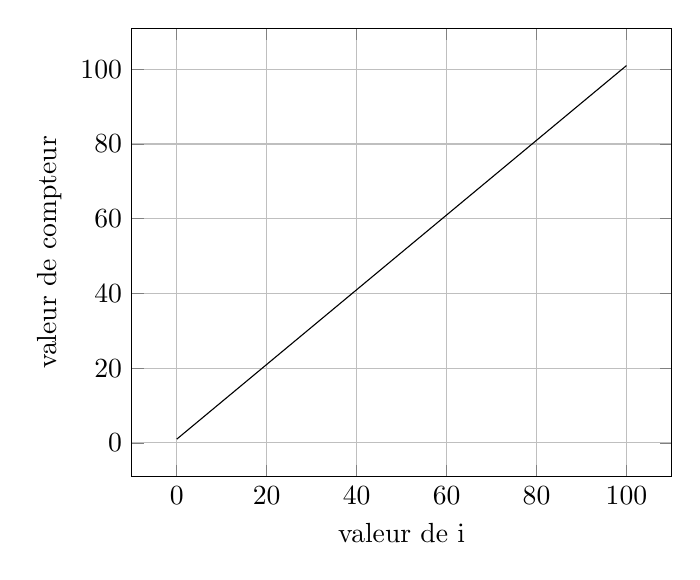
\begin{tikzpicture}
		\begin{axis}[domain=0:100,grid=major,xlabel=valeur de i,ylabel = valeur de compteur]
			\addplot[no markers]{x+1};
		\end{axis}
	\end{tikzpicture}
	\caption{Courbe de i en fonction de compteur}
	\end{figure}
	
	
	\item Boucle \lstinline|while| : Idéale pour un nombre défini d'itérations.
	
	\ex{While}
	\lstinputlisting[linerange={56-60}]{Code/Instructions.cpp}
	
	\item Boucle \lstinline|do while| : Idéale pour un nombre défini d'itérations.
	
	\ex{Do/While}
	\lstinputlisting[linerange={62-72}]{Code/Instructions.cpp}
\end{itemize}